\chapter{绪论}\label{chap:intro}

\section{研究背景与意义}
2000至今,计算机领域有着跨越式的发展\citet{bhosale2014review}。计算机系统已经不仅仅应用于科研、银行、企业等领域,而是融入了每一个人的日常生后之中。从计算机软硬件系统的角度来看,计算机系统由传统的IOE架构,也就是IBM公司生产的小型机,Oracle公司研发的数据库软件,EMC公司研发的高端商用存储发展 成为扩展性、性价比更高的分布式架构。传统IOE架构存在着扩展性差,硬件成本高的问题。这些问题就使得IOE架构无法满足2000年以后蓬勃发展的互联网应用的需求。

为了满足互联网应用数据量大,增长迅速、成本要求严格的要求。各个公司研发了一系列基于廉价硬件的分布式软件系统。其中谷歌公司于2003年至2006年发表的三篇论文:GFS\cite{ghemawat2003google},MapReduce \cite{dean2008mapreduce} 以及BitTable \cite{chang2008bigtable} 对引领了整个分布式系统领域的发展。GFS(Google File System)这篇论文介绍了分布式文件系统的设计与实现,GFS最大的特点是具有良好的可扩展性,支持大文件存储,并且运行在廉价硬件上,通过多副本的方式提供了容错性,从根本原理上来说,GFS将一个大文件切成很多小块,每一小块数据存储在多个磁盘中,GFS系统解决了大规模数据的存储问题。MapReduce介绍了处理大数据的方法,通过将任务分发到多个计算节点同时计算,最后在Reduce阶段汇总结果从而完成大数据处理。BigTable解决的结构化数据的存储问题。这三篇论文解决了分布式大数据处理领域最核心的三个问题,也启发了众多分布式系统的发展。

在数据处理这一个领域,在2004年MapReduce发表之后,各个公司实验室研发了一系列的数据处理系统。比如雅虎公司研发并开源了Hadoop\cite{white2012hadoop}、HDFS\cite{shvachko2010hadoop}、Hbase\cite{vora2011hadoop}三个系统,分别对应MapReduce、GFS、BitTable三个系统。后面基于Hadoop也有一系列的该进。比如Pig、Hive\cite{thusoo2009hive}系统添加了对脚本语言和SQL\cite{armbrust2015spark}查询语言的支持。微软和阿里巴巴等公司也研发了Dryad\cite{isard2007dryad},Scopt\cite{chaiken2008scope}、Fuxi\cite{zhang2014fuxi}等大数据系统。这些系统虽然可以处理大规模数据,但是因为要将中间数据存储在HDFS\cite{shvachko2010hadoop},使得计算速度很慢,也无法满足机器学习,图计算等迭代计算作业的要求。为了解决这些问题,加州大学伯克利分校的AMPLab研发了基于内存计算的分布式数据处理系统Spark\cite{zaharia2010spark},它的主要特点是将中间数据存储在内存之中,这样就可以极大的加快数据处理的速度。和传统的Hadoop系统对比,在Spark的优势项目迭代式计算方面,有着上百倍的性能提\cite{gopalani2015comparing}。在作业执行的灵活性上,Spark也做出了很大的该进。比如在执行的过程中,Spark框架会根据运行时的作业信息动态调整作业的执行计划。比如在发生了数据倾斜的情况时,Spark会创建多个task计算大的分区的数据,在处理完毕之后会添加一个union操作合并数据\cite{zaharia2010spark}。

对比Hadoop和Spark就会发现,缓存管理系统是Spark相对于Hadoop做出的核心改进。在Spark系统之中,可以在作业执行节点缓存数据,缓存数据的决策是由编程人员实现的。编程人员在编写Spark代码的过程中,如果发现数据会多次访问到,就会调用cache接口缓存数据。调用cache接口之后,spark系统会设置数据的缓存标志为memory,在计算的过程中,经过计算得到数据之后,spark系统会检查缓存标志,根据缓存标志将数据存放在不同位置,比如内存,磁盘或者直接丢弃。这种缓存策略需要编程人员手动指定缓存位置,会在一定程度上增加编程人员的开发负担,减慢软件的开发进度。

另一个方面,对于缓存数据的管理方面,spark使用的是LRU缓存替换策略管理缓存数据。LRU这种策略非常简单,在缓存空间不够用的时候会替换最近没有访问过的数据。这种缓存替换策略是不适合Spark这种复杂的应用场景的。因为Spark作业会生成一个复杂的计算图,计算图中每个节点是数据,每个数据都需要根据计算图的拓扑结构一步步计算得来,每个数据的计算代价也是完全不同的。可见每个节点的数据并不相等,有的数据可以很快重新计算得到,有的数据如果丢失重新计算它的开销是非常大的。而LRU缓存替换策略只考虑了数据访问的时间信息,这就有可能将重新计算开销非常大的数据替换出去,造成作业执行速度变慢。

\section{课题研究内容}

本文将从两个大的方面进行研究。第一个方面,研究Spark自动缓存系统。第二个方面,研究优化Spark缓存管理策略。对于自动缓存系统,本文使用了一种改进的基于二次执行的自动缓存系统。对于缓存管理方面,本文使用了一种容错性加强的缓存清理策略和一种针对Spark系统特点设计的缓存替换策略。

\begin{enumerate}
    \item 对于自动缓存系统,当前的Spark系统需要手动指定缓存数据,这会加大编程人员的思考负担,在程序规模很大的情况下,思考数据使用情况,数据大小,考虑缓存数据是一件很麻烦的事情。所以需要Spark框架能够自动检测需要缓存的数据,做出缓存决策,减轻编程人员的负担。同时还需考虑Spark框架的新特性,因为Spark有动态执行的新特性,自动缓存模块也需要在Spark框架动态执行调整执行计划的时候同时针对性地做出调整,做出正确的缓存决策。
    \item 针对缓存管理模块,目前因为Spark系统使用JVM(Java Virtual Machine)运行,框架与JVM的内存管理是完全隔离的,这就有可能导致JVM的OOM(Out of Memory)错误。为了解决这个潜在的问题,就需要自动清理缓存中的数据。为了保证容错性,在清理数据的时候需要保存一定的冗余,这样在发生错误的时候就可以通过冗余数据恢复计算。所以就需要根据Spark框架的实现原理,合理设计并实现缓存数据的清理功能。对于缓存替换策略,也需要根据Spark框架的原理设计合适的缓存策略。本文根据Spark计算图的拓扑结构以及计算过程中得到的数据综合计算数据权重,根据数据权重从低到高替换数据。提升整个作业的执行速度。
\end{enumerate}

\section{相关工作}
针对Spark系统的优化主要集中在框架优化\cite{罗妮0基于机器学习的内存计算优化关键技术研究}\cite{廖湖声0Spark},参数配置优化\cite{范天文2020基于内存计算框架},Shuffle优化\cite{cheng2020ops}\cite{choi2015early}\cite{davidson2013optimizing}\cite{stone1971parallel}\cite{furukawa2001efficient}\cite{liu2017optimizing}\cite{张伟0Spark}\cite{lu2014accelerating},任务调度优化\cite{杨志伟2016异构}\cite{李源0Spark},缓存优\cite{kim2017sparkle}化\cite{卞琛2017并行计算框架}\cite{陈康2016Spark}这五个方面。下文会对缓存优化进行详细介绍,对其他四个方面也会进行简单的介绍。

对于框架优化,一般是对Spark框架本身进行一系列的优化,对于Spark中的算子就有很多优化方式。比如文献\cite{罗妮0基于机器学习的内存计算优化关键技术研究}提供了一种新的join方式ApproxJoin,就可以显著提升join操作的效率。英伟达改造了算子的底层实现方式,使用GPU加速算子的执行过程\cite{廖湖声0Spark}。

对于参数配置优化,是通过调整参数为Spark框架提供合适的运行环境,合理的参数配置会使得Spark框架能够充分利用机器资源。这方面主要通过HBO(History Based Optimization)基于历史统计信息的优citet{范天文2020基于内存计算框架}化。也有文献将机器学习和参数优化结合起来,提出了一种基于决策树的参数优化方法\cite{罗妮0基于机器学习的内存计算优化关键技术研究}。

对于Shuffle优化,因为上有节点的数据需要通过Shuffle才能被下游计算节点使用,Shuffle节点会阻塞计算图下游节点的运行。所以Shuffle性能的高低对于整个作业的性能和吞吐量有着巨大的影响。所以有很多针对Shuffle的优化方法。正对Shuffle过程中数据倾斜问题,有文献\cite{cheng2020ops}提出一种针对数据倾斜数据块的优化算法,通过调整shuffle输出的临时文件来改善Shuffle运行时间。还有通过分布式内存优化Shuffle的Alluxio系统\cite{li2018alluxio}(也称为Tachyon\cite{li2014tachyon})等。

对于任务调度优化,文献\cite{zaharia2016architecture}提出了一种可以同时解决数据局部性和调度公平性的延迟调度算法。杨志伟等人提出了一种针对异构Spark计算集群的自适应任务调度策略(Heterogeneous Spark Adaptive Task Scheduling, HSATS),HSATS的主要思想是实时检测集群中的状态,并根据状态信息调整作业的分配权重信息,使用权重信息进行任务调度。启发式的算法也被大量应用于异构计算集群作业调度优化领域,例如文献中设计了针对异构计算集群的任务感知调度系统RUPAM,RUPAM使用了一种启发式的算法,根据异构集群的多种特征进行作业调度优化。

此外还有对容错性等方面的研究。Spark默认使用checkpoint机制和数据血缘机制实现容错功能。checkpoint是通过将重要数据数据持久化到磁盘之中实现\cite{ananthanarayanan2012pacman}。血缘机制通过DAG图信息重复计算丢失数据实现容错功能\cite{zaharia2010spark}。文献\cite{zaharia2012resilient}提出了应用级别的容错机制,应用会在执行过程中自动设置checkpoint,将数据存储到新型非易失性存储实现容错恢复功能。文献\cite{dimitriou2015retrial}提出了一种系统级别的checkpoint恢复机制。该方法的特点是对用户完全透明,通过硬件实现容错恢复功能。

\subsection{分布式系统内存管理}

在分布式场景中,大量作业共享计算集群。合理高效的利用计算集群的计算资源不仅对于单个作业的运行性能有着重大影响,同时也成为提高计算集群能效比的关键。所以分布式系统中的资源管理和分配是分布式云场景下需要研究的重要问题。在资源调度管理中,分布式集群的内存管理是分布式系统资源管理和优化的核心问题,尤其对于Spark分布式系统来说,因为Spark是基于内存的分布式计算系统,所以内存管理是提升Spark性能的关键。

Hadoop通过一种静态固定的资源槽(slot)方式管理处理器以及内存资源。Slot中包含一定数量的CPU和内存资源。Hadoop集群资源控制器将整个系统资源分成固定数量的slot,每个slot可以运行一个Map作业或者一个Reduce作业。Hadoop通过slot的方式简化了对资源的管理,运行过程中只需要将slot分配个任务。有很多针对Hadoop这种基于slot的资源管理方式的研究。Jord`a Polo根据Hadoop中运行的作业特点,动态调整slot的数量和资源量,从而可以提高集群的资源利用率。Jord`a Polo还提出了一种保证性能的前提下提高资源利用率的资源调度算法。具体来说会检测当前集群中作业的性能,在满足性能的前提下分配尽量少的资源,从而可以提升集群的资源利用率。

Haoyuan Li实现了Tachyon\cite{li2014tachyon}(改名为Alluxio\cite{li2018alluxio}),Alluxio是一个分布式内存文件系统,位于计算框架与文件系统之间,主要作为文件系统的缓存优化读取速度。比如计算框架的不同作业之间需要交换数据时,一般是通过将数据写入分布式文件的临时文件中,并将文件地址发送给另一个作业,这就会造成很大的文件存取延迟。通过使用Alluxio作为文件系统的缓存,任务将数据写入分布式内存文件系统缓存Alluxio之中,这样就可以避免缓慢的文件系统读取延迟,加速作业的执行速度。不同的任务需要读取同一个文件的时候,也可以将数据缓存在Alluxio内存之中,从而可以避免重复加载文件。Alluxio的这些特性使得它可以极大地提高HDFS的读写速度。也可以让作业端到端执行速度加速4倍。

Bikash Sharma提出了一种细粒度的资源分配策略MROrchestrator\cite{6253482}。MROrchestrator改变了Hadoop传统的基于slot的的资源分配方式,因为这种方式每个作业只能使用一个slot内部的处理器以及内存资源。Hadoop集群要根据集群的情况创建多种不同的slot。这种静态的资源分配方式无法很好的满足任务多种多样的资源需求。所以MROrchestrator会检测每个作业的负载情况,并实时做出调整。从而能够更高效率地利用系统资源。相对于静态的基于slot的资源分配方式,MROrchetrator动态资源分配机制可以使作业的平均执行时间减少38\%。集群资源使用效率平均提升25\%。

Daniel Warneke等人的研究表明\cite{5710902},MapReduce这一类作业具有内存弹性的特点。内存弹性是指内存空间越多,任务的执行速度也会相应变快。内存总量减少并不会导致作业运行出错,只是会让作业执行速度变慢。所以他们提出了一种动态资源申请方法。作业开始执行是会想系统申请作业可以执行的最小资源,称之为保证型共享内存(guaranteed share memory),保证型共享内存在作业运行过程中是保持不变的。除此之外还提出了给予型共享内存(granted share memory)。作业在运行过程中如果需要更多的内存,就可以向集群资源管理器申请给予型共享内存。集群资源管理器根据集群的运行状态决定是否分配资源。当新的作业提交到系统,需要保证型共享内存才能执行任务,集群资源管理器就会回收集群的给予型共享内存。这种动态调度方式可以在保证集群作业公平性的前提下提升集群中内存的使用效率。

Feng Lin等\cite{冯琳0集群计算引擎}认为,Spark将RDD缓存的工作全都交给编程人员会有潜在的问题。第一,编程人员如果缓存了不必要的数据会造成内存浪费。第二,编程人员如果遗漏了重要数据,没有缓存,会影响到作业的执行速度。第三,程序规模变大时,会给编程人员带来很大的额外负担。所以他们设计了一种自动缓存系统。但是这种策略适用于静态计算图,在新版本的Spark中具有自适应动态执行的特性(Adaptive Execution),这种基于静态计算图的自动缓存方法需要进一步改进。

\subsection{分布式系统缓存替换策略研究}

缓存替换技术主要分为三类,第一类是传统缓存替换技术,第二类是多级缓存替换技术,第三类是代价缓存替换技术。传统缓存替换技术一般只关注缓存的访问时间和使用频率。比如常见的传统缓存替换技术有LRU(Least Recently Used)最近最少使用算法、LFU(Least Frequently Used)最不经常使用算法等。Spark就使用LRU作为其缓存替换策略,这类传统缓存替换策略比较简单,考虑的因素比较单一,在复杂场景下做出的缓存替换策略可能会不太合理。

多级缓存替换技术是在传统缓存技术的基础上发展来的,一般有多个缓存队列。比如K级最近最少使用算法(LRU-K\cite{o1993lru})、有一个FIFO队列和一个LRU队列组成的双队列算法(Two Queues,2Q\cite{dimitriou2015retrial})、多级队列缓存替换算法(Multi-Queue,MQ\cite{li2015sparkbench})。

代价缓存策略会根据作业的特点和集群的状态综合计算作业的权重,从而可以兼顾作业的运行速度和集群的资源利用率。Y.Z.Geng等人\cite{geng2014simulation}提出了LCS策略,这种策略通过分析作业的依赖关系,根据作业丢失产生的恢复成本决定数据的权重。这种方式可以避免将恢复代价很大的数据替换出缓存,从而可以避免作业运行速度下降。还有人将集群资源利用率,作业执行时间等统一建模为能量函数,将问题转化为数值优化问题,通过优化算法计算是的能量函数最大的数据权重值。

\section{本文的主要工作}

本文主要研究分布式内存计算框架Spark的缓存优化技术,主要针对Spark框架的新特性,研究自动缓存技术。以及缓存管理技术,从而可以提高作业的执行速度。本文将从以下四个方面进行研究:

\begin{enumerate}
    \item 研究研究分析分布式内存计算系统Spark的设计实验机制、资源管理方式和作业调度运行模式。测试并分析Spark内存管理机制的特点和问题。Hadoop和Spark都是基于Map-Reduce编程模式的分布式计算系统。Spark性能优于Hadoop的一个很重要的原因就是Spark的内存管理机制。研究分析Spark的内存管理机制有助于进一步优化Spark系统和Spark应用。计划使用中科院大数据测试BigDataBench数据集测试Spark框架中Shuffle Memory和Storage Memory内存分区的使用特点。
    \item 设计实现针对Spark3.0的自动缓存系统。之前的工作自动缓存工作是通过提前运行小规模数据集得到重复使用的RDD数据,之后再执行大规模数据集时自动缓存重复使用的RDD数据。然而2020年6月发布的Spark3.0添加了动态执行特性。框架会在执行过程中根据数据特点选择合适的执行策略。这就要求需要在运行过程中实时监测应该缓存的RDD数据。
    \item 设计实现一种Spark系统中的缓存替换策略。目前Spark系统中使用的是LRU缓存替换策略。LRU策略仅仅能够利用内存中数据访问的时间特性。Spark系统的内存中存储的RDD还具有分布式存储、大小、计算代价等其他特征。所以需要综合考虑RDD数据的特征以及整个作业的拓扑特征,综合考虑,淘汰其中权值最小的RDD数据。
    \item 缓存清理算法。Spark内存管理依赖与JVM(JAVA虚拟机)内存管理。因为Spark executor是一个JVM进程。使用了固定大小的JVM堆内存。Spark框架和JVM堆内存管理是完全隔离的,Spark框架自身会记录内存使用量。在内存不足时会删除内存中缓存的RDD数据,删除操作仅仅是删除内存对象的引用。实际内存回收依赖于JVM的内存回收机制。JVM定期检测内存对象的引用计数,如果引用计数减少为0说明内存对象可以回收,JVM就会进行实际的内存回收。所以Spark如果发生了缓存替换,JVM内存并未回收的情况就会产生OOM(Out of Memory)错误。所以就需要Spark框架自动提前删除不需要的缓存对象,提高内存空间利用率。在清理的同时也要更具作业的拓扑信息保存一定的冗余信息,以便于作业执行出错时能够使用冗余信息迅速恢复计算。
\end{enumerate}

\section{论文结构}

论文的组织结构如下,各章的逻辑关系如图:

第一章:绪论。主要阐述研究背景和研究意义,并分析了国内外相关研究的现状,介绍了本文的主要工作和文章结构。

第二章:分布式大数据内存计算系统Spark系统实现机制概述。本章会分析阐述Spark系统架构以及任务调度执行流程。重点介绍缓存实现原理和缓存管理机制。并且通过实验分析了缓存管理对任务执行速度造成的影响。

第三章:Spark自动缓存模块设计与实现。本章会阐述自动缓存模块的设计以及实现方法。之前的工作,不适用于目前新版本的动态执行框架,本文提出了一种实时自动缓存框架,最后通过实验对比分析了自动缓存框架的性能。

第四章:一种基于DAG作业运行时信息及拓扑结构的缓存替换策略的设计与实现。本章会提出一种结合了作业DAG拓扑结构以及作业执行信息的缓存计算方法。这种方法综合考虑了多种信息,避免了目前框架使用的LRU算法存在的可能将重要数据替换删除的问题。最后通过实验验证了这种缓存替换策略相对于LRU策略的有效性。

第五章:一种容错性加强的自动缓存清理方法。对于分布式系统,必须要重点保证容错信。对于分布式内存计算系统Spark,它的容错原理是在出错情况下根据DAG拓扑重复计算上游数据。所以如果在出错场景下有可能会造成重复计算,导致任务执行延迟。为了避免这种问题,本文采用了以时间换空间的原理,在缓存中保存一定的冗余信息,在出错场景可以迅速通过冗余信息恢复计算。

第六章:总结与展望。本章总结论文的主要内容,并展望后续工作。

\begin{figure}
    \centering
    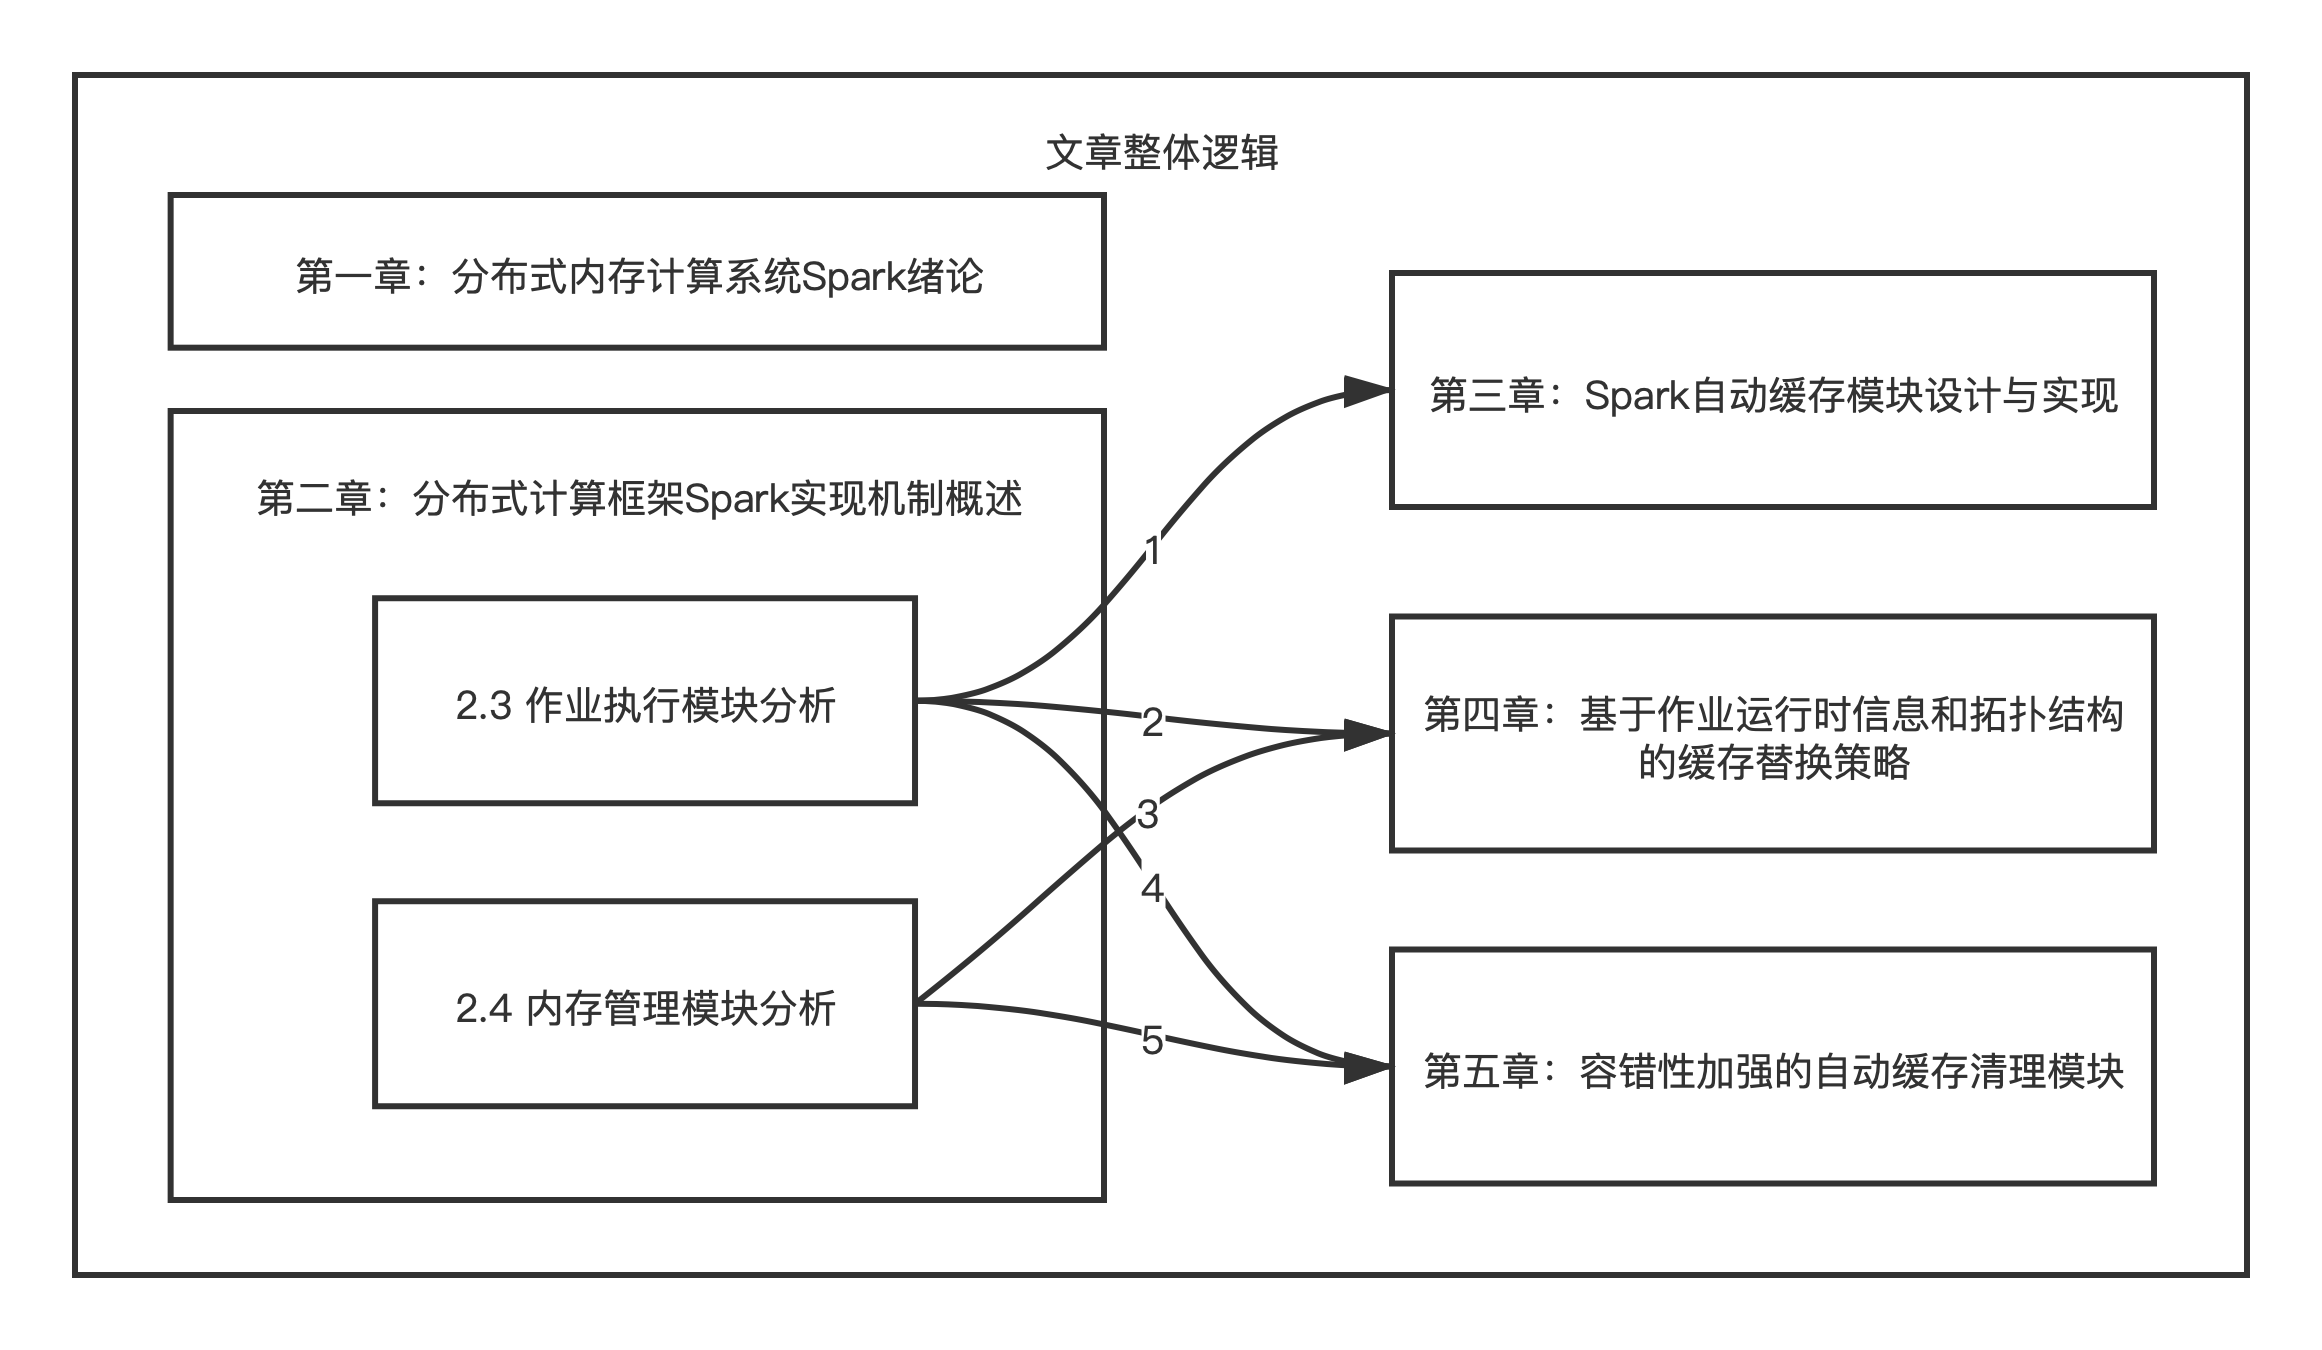
\includegraphics[width=0.99\textwidth]{Img/毕业设计整体逻辑.png}
    \caption{文章整体逻辑}
    \label{fig:paper-logic}
\end{figure}